\documentclass[xetex,mathserif,serif]{beamer}
\usepackage{polyglossia}
\setdefaultlanguage[babelshorthands=true]{russian}
\usepackage{minted}
\usepackage{tabu}

\useoutertheme{infolines}

\usepackage{fontspec}
\setmainfont{FreeSans}
\newfontfamily{\russianfonttt}{FreeSans}

\tabulinesep=0.7mm

\title{Предметно-ориентированное проектирование}
\subtitle{Domain-Driven Design}
\author[Юрий Литвинов]{Юрий Литвинов \newline \textcolor{gray}{\small\texttt{yurii.litvinov@gmail.com}}}

\date{23.04.2019г}

\begin{document}
	
	\frame{\titlepage}

	\section{Введение}

	\begin{frame}
		\frametitle{Domain-Driven Design}
		\textbf{Domain-Driven Design} --- модная нынче методология проектирования, использующая предметную область как основу архитектуры системы
		\begin{itemize}
			\item Архитектура приложения строится вокруг \textbf{Модели предметной области}
			\item Модель определяет \textbf{Единый язык}, на котором общаются и разработчики, и эксперты, описывая естественными фразами то, что происходит и в программе, и в реальности
			\item Модель --- это не только диаграммы, это ещё (и прежде всего) код, и устное общение
		\end{itemize}
		DDD даёт ответ на вопрос ``откуда брать эти все классы'' и позволяет целенаправленно уточнять и улучшать архитектуру системы. 
		Особенно полезно, когда предметная область не очень знакома.
	\end{frame}

	\begin{frame}
		\frametitle{Книжка}
		Эрик Эванс, ``Предметно-ориентированное проектирование. Структуризация сложных программных систем''. М., ``Вильямс'', 2010, 448 стр.
		\begin{center}
			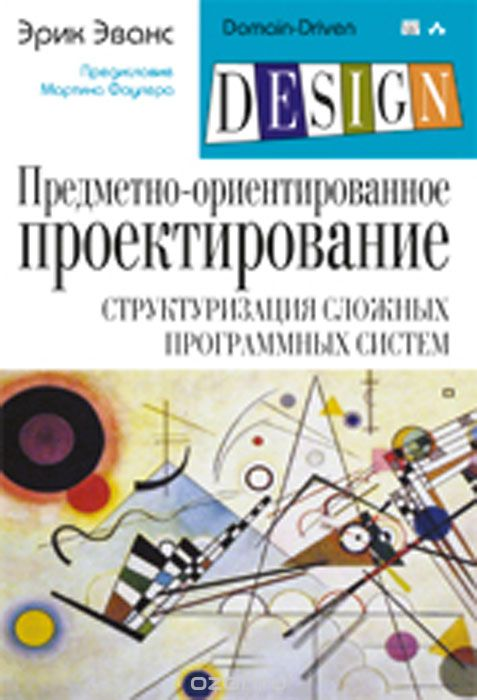
\includegraphics[width=0.25\textwidth]{dddCover.jpg}
		\end{center}
	\end{frame}

	\section{Пример}

	\begin{frame}
		\frametitle{Domain-Driven Design, анализ}
		\framesubtitle{Пример: печатные платы}
		\begin{center}
			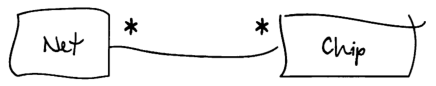
\includegraphics[width=0.6\textwidth]{netClasses.png}

			\bigskip

			\bigskip
			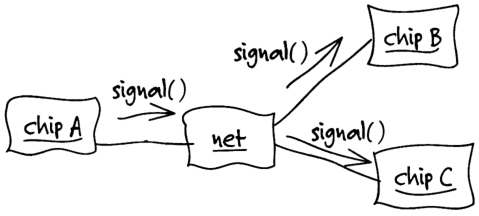
\includegraphics[width=0.6\textwidth]{netObjects.png}
		\end{center}
	\end{frame}

	\begin{frame}
		\frametitle{Печатные платы, топология}
		\begin{center}
			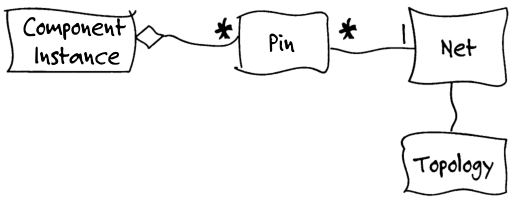
\includegraphics[width=0.7\textwidth]{topology.png}
		\end{center}
	\end{frame}

	\begin{frame}
		\frametitle{Печатные платы, сигналы}
		\begin{center}
			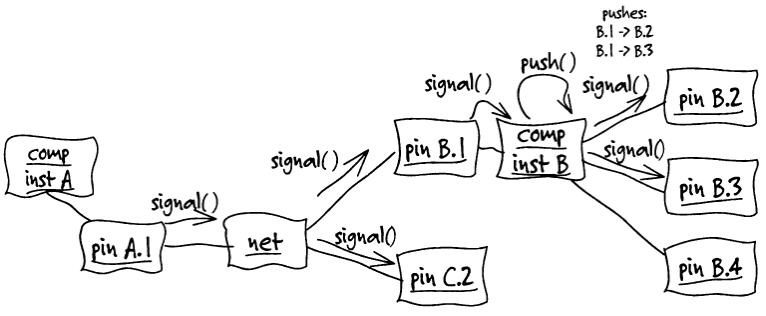
\includegraphics[width=0.9\textwidth]{signals.png}
		\end{center}
	\end{frame}

	\begin{frame}
		\frametitle{Печатные платы, прозванивание}
		\begin{center}
			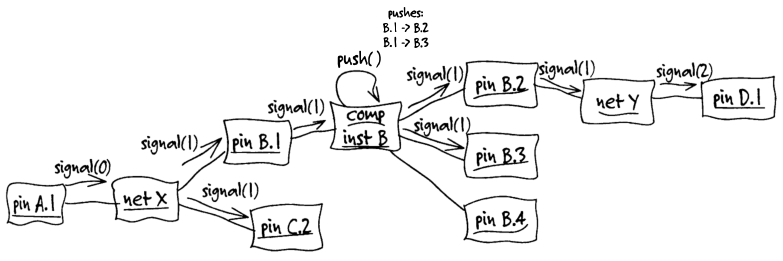
\includegraphics[width=\textwidth]{probeSimulation.png}
		\end{center}
	\end{frame}

	\begin{frame}
		\frametitle{Печатные платы, типы}
		\begin{center}
			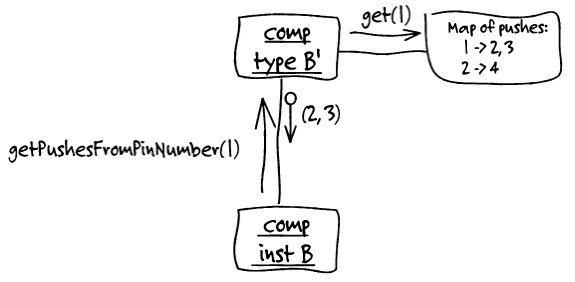
\includegraphics[width=0.7\textwidth]{types.png}
		\end{center}
	\end{frame}

	\begin{frame}
		\frametitle{Печатные платы, модель}
		\begin{center}
			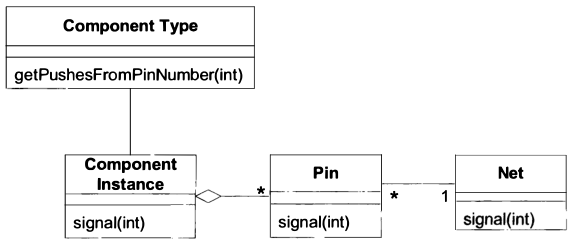
\includegraphics[width=0.8\textwidth]{finalModel.png}
		\end{center}
	\end{frame}

	\begin{frame}
		\frametitle{Выводы: правила игры}
		\begin{itemize}
			\item Детали реализации не участвуют в модели
			\begin{itemize}
				\item ``База данных? Какая база данных?''
			\end{itemize}
			\item Должно быть можно общаться, пользуясь только именами классов и методов
			\item Не нужные для текущей задачи сущности предметной области не должны быть в модели
			\item Могут быть скрытые сущности, которые следует выделить явно
			\begin{itemize}
				\item при этом объяснив экспертам их роль в реальной жизни и послушав их мнение
				\item например, различные ограничения могут стать отдельными классами
			\end{itemize}
			\item Диаграммы объектов могут быть очень полезны
		\end{itemize}
	\end{frame}

	\section{Единый язык}

	\begin{frame}
		\frametitle{``Моделирование вслух''}
		\textit{Если передать в \textbf{Маршрутизатор} пункт отправки, пункт назначения, время прибытия, то он найдет нужные остановки в пути следования груза, а потом, ну... запишет их в базу данных.}

		\vspace{3mm}

		\textit{Пункт отправки, пункт назначения и все такое... все это идет в \textbf{Маршрутизатор}, а оттуда получаем \textbf{Маршрут}, в котором записано все, что нужно.}

		\vspace{3mm}

		\textit{\textbf{Маршрутизатор} находит \textbf{Маршрут}, удовлетворяющий \textbf{Спецификации маршрута}.}
	\end{frame}

	\section{Модель, основные шаблоны}

	\begin{frame}
		\frametitle{Изоляция предметной области}
		\begin{center}
			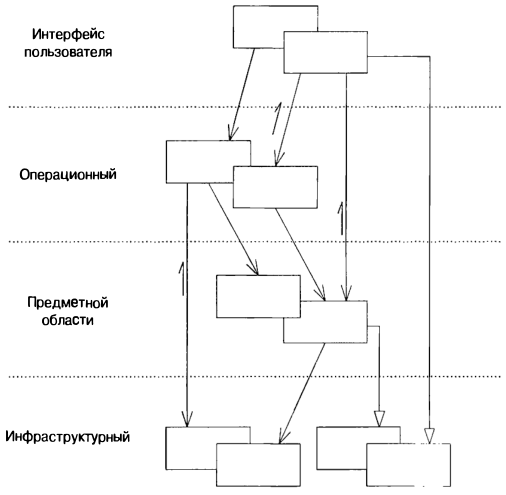
\includegraphics[height=0.8\textheight]{layers.png}
		\end{center}
	\end{frame}

	\begin{frame}
		\frametitle{Основные структурные элементы модели}
		\begin{itemize}
			\item \textbf{Сущность (Entity)} --- объект, обладающий собственной идентичностью
			\begin{itemize}
				\item Нужна операция идентификации
				\item Нужен способ поддержания идентичности
			\end{itemize}
			\item \textbf{Объект-значение (Value object)} --- объект, полностью определяемый своими атрибутами
			\begin{itemize}
				\item ``Лучше'', чем сущность
				\item Как правило, немутабельны
				\item Могут быть разделяемыми
			\end{itemize}
			\item \textbf{Служба (Service)} --- объект, представляющий операцию
			\begin{itemize}
				\item Как правило, не имеет собственного состояния
				\item Операции нет естественного места в других классах модели
			\end{itemize}
			\item \textbf{Модуль (Module)} --- смысловые части модели
		\end{itemize}
	\end{frame}

	\begin{frame}
		\frametitle{Агрегаты}
		\begin{itemize}
			\item \textbf{Агрегат} --- изолированный кусок модели, имеющий \textbf{корень} и \textbf{границу}
			\item Корень --- глобально идентичный объект-сущность
			\item Остальные объекты в агрегате идентичны локально
			\item Извне агрегата можно хранить ссылку только на корень
			\begin{itemize}
				\item Отдавать временную ссылку можно
			\end{itemize}
			\item Корень отвечает за поддержание инвариантов всего агрегата
		\end{itemize}
	\end{frame}

	\begin{frame}
		\frametitle{Агрегат, пример}
		\begin{center}
			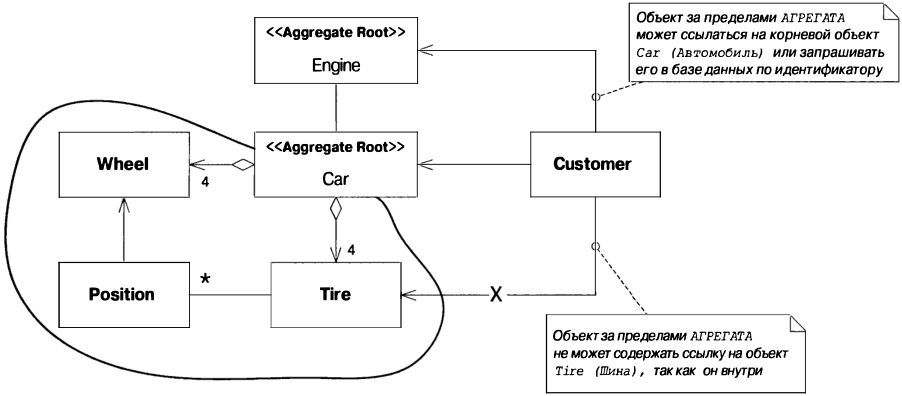
\includegraphics[width=0.9\textwidth]{aggregate.png}
		\end{center}
	\end{frame}

	\begin{frame}
		\frametitle{Фабрика}
		\begin{center}
			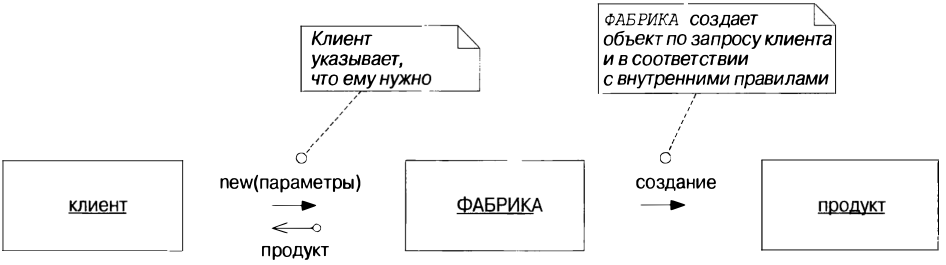
\includegraphics[width=0.7\textwidth]{factory.png}
		\end{center}
		\textbf{Фабрика} служит для создания объектов или агрегатов
		\begin{itemize}
			\item Скрывает внутреннее устройство конструируемого объекта
			\begin{itemize}
				\item Операция создания ``атомарна'' и обеспечивает инварианты
			\end{itemize}
			\item Изолирует сложную операцию создания
			\item Как правило, не имеет бизнес-смысла, но является частью модели
			\item Реализуется аж несколькими разными паттернами
		\end{itemize}
	\end{frame}

	\begin{frame}
		\frametitle{Пример}
		\framesubtitle{Фабрика, использующаяся для восстановления объекта}
		\begin{center}
			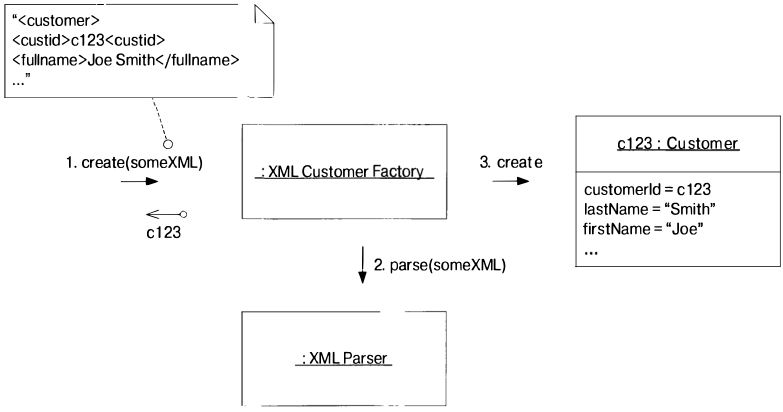
\includegraphics[width=0.8\textwidth]{xmlFactory.png}
		\end{center}
	\end{frame}

	\begin{frame}
		\frametitle{Хранилище (Repository)}
		\begin{center}
			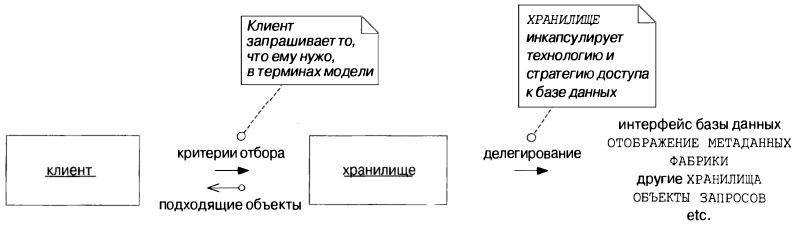
\includegraphics[width=0.8\textwidth]{repository.png}
		\end{center}
		\textbf{Репозиторий} хранит объекты и предоставляет к ним доступ
		\begin{itemize}
			\item Может инкапсулировать запросы к БД
			\item Может использовать фабрики
			\item Может обладать развитым интерфейсом запросов
		\end{itemize}
	\end{frame}

	\section{Моделирование ограничений}

	\begin{frame}
		\frametitle{Моделирование ограничений}
		\framesubtitle{Простой пример}
		\begin{center}
			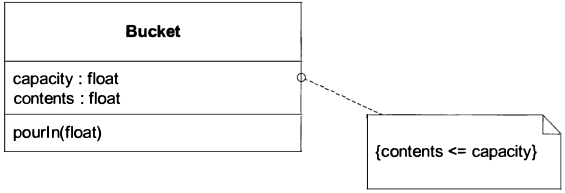
\includegraphics[width=0.6\textwidth]{bucket.png}
		\end{center}
	\end{frame}

	\begin{frame}[fragile]
		\frametitle{Код, до}
		\begin{minted}{java}
class Bucket {
    private float capacity;
    private float contents;

    public void pourIn(float addedVolume) {
        if (contents + addedVolume > capacity) {
            contents = capacity;
        } else {
            contents = contents + addedVolume;
    }
}
		\end{minted}
	\end{frame}

	\begin{frame}[fragile]
		\frametitle{Код, после}
		\begin{minted}{java}
class Bucket {
    private float capacity;
    private float contents;

    public void pourIn(float addedVolume) {
        float volumePresent = contents + addedVolume;
        contents = constrainedToCapacity(volumePresent);
    }

    private float constrainedToCapacity(float volumePlacedIn) {
        if (volumePlacedIn > capacity) return capacity;
        return volumePlacedIn;
    }
} 
		\end{minted}
	\end{frame}

	\begin{frame}
		\frametitle{Паттерн ``Спецификация''}
		\begin{center}
			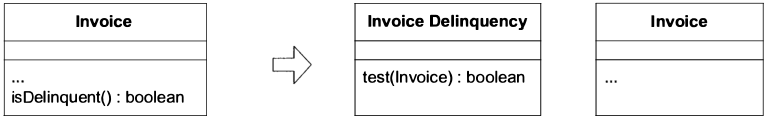
\includegraphics[width=0.8\textwidth]{specification.png}
		\end{center}
		\textbf{Спецификация} инкапсулирует ограничение в отдельном объекте
		\begin{itemize}
			\item Предикат
			\item Может быть использована для выборки или конструирования объектов
		\end{itemize}
	\end{frame}

	\begin{frame}
		\frametitle{Композитные спецификации}
		\begin{center}
			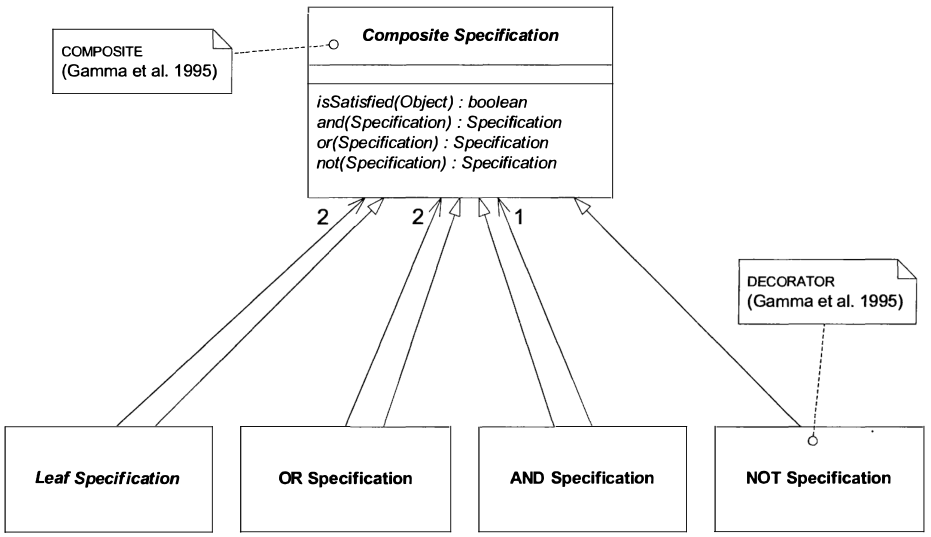
\includegraphics[height=0.7\textheight]{compositeSpecifications.png}
		\end{center}
	\end{frame}

	\begin{frame}
		\frametitle{Пример: склад химикатов}
		\begin{center}
			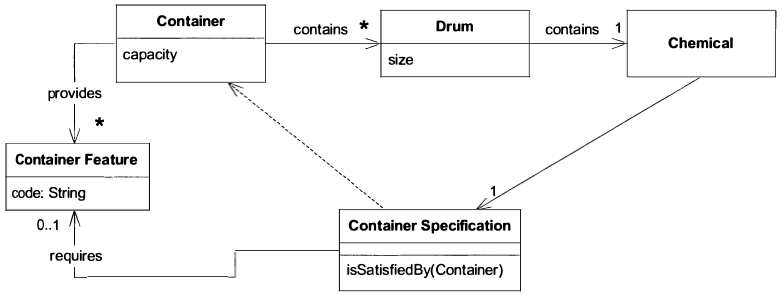
\includegraphics[width=0.9\textwidth]{chemicalsStructure.png}
		\end{center}
	\end{frame}

	\begin{frame}[fragile]
		\frametitle{Код, спецификация}
		\begin{minted}{java}
public class ContainerSpecification {
    private ContainerFeature requiredFeature;

    public ContainerSpecification(ContainerFeature required) {
        requiredFeature = required;
    }

    boolean isSatisfiedBy(Container aContainer) {
        return aContainer.getFeatures().contains(requiredFeature);
    }
}
		\end{minted}
\end{frame}

	\begin{frame}[fragile]
		\frametitle{Код, контейнер}
		\begin{minted}{java}
boolean isSafelyPacked() {
    Iterator it = contents.iterator();
    while (it.hasNext()) {
        Drum drum = (Drum) it.next() ;
        if (!drum.containerSpecification().isSatisfiedBy(this))
            return false ;
    }
    return true;
}
		\end{minted}
	\end{frame}

\end{document}
